\chapter{The first application}


\section{A bit of terminology}

CLIM was developed before the GUI toolkits widely used at the moment.
Qt, GTK and others appeared much later than CLIM and the difference of
terminology reflects this.

A CLIM application is made up of a hierarchy of an \gloss{application
  frame}, \gloss{panes} and \gloss{gadgets} (gadgets are special kinds
of panes):

\begin{itemize}
\item
  An \emph{application frame} is what would usually be called an
  application.

\item
  At a very high level, panes describe an application frame's visual
  building blocks: a side bar, a menu bar, a table displaying a list
  of items, a text input are all panes. They can be used by
  application programmers to compose the top-level user interface of
  their applications, as well as auxiliary components such as menus
  and dialogs. In addition, panes can be more abstract such as layout
  panes such as \pane{hbox}, \pane{vbox} to arrange other panes
  horizontally or vertically, etc.

\item
  \emph{gadgets} correspond to what other toolkits call \emph{widgets}
  and \emph{control}.  Frequently used CLIM gadgets are
  \gadget{button}s, \gadget{slider}s, etc.
\end{itemize}


\section{How CLIM applications produce output}

Although it is easy to imagine panes in terms of their appearance on
screen, they are much richer: they are actually the series of
operations that produces that appearance. They are not only the end
product visible on a screen, but they contain all the step-by-step
information that led to that representation.

More precisely, CLIM panes record the series of operations that
generates an output.  This means that such a pane maintains a display
list, consisting of a sequence of output records, ordered
chronologically, from the first output record to be drawn to the last.

This display list is used to fill in damaged areas of the pane, for
instance as a result of the pane being partially or totally covered by
other panes, and then having some or all of its area again becoming
visible.  The output records of the display list that have some parts
in common with the exposed area are partially or totally replayed (in
chronological order) to redraw the contents of the area.

An application can have a pane establish this display list in several
fundamentally different ways, each more sophisticated:

\begin{description}
  \item[Simple application:] Very simple applications have no internal
    data structure to keep track of application objects, and simply
    produce output to the pane from time to time as a result of
    running commands, occasionally perhaps erasing the pane and
    starting over.  Such applications typically use text or graphics
    output as a result of running commands.  CLIM maintains the
    display list for the pane, and adds to the end of it, each time
    also producing the rendering instructions \footnote{rendering is
      carried out by a backend. X11 is currently the standard
      backend.} that result from drawing the new output record.  If
    the pane uses scrolling (which it typically does), then CLIM must
    determine the extent of the pane so as to update the scroll bar
    after each new output.

  \item[Application with a static display function:] More complicated
    applications use a display function.  Before the display function
    is run, the existing display list is typically deleted, so that
    the purpose of the display function becomes to establish an
    entirely new display list.  The display function might for
    instance produce some kind of form to be filled in, and
    application commands can use text or graphics operations to fill
    in the form.  A game of tic-tac-toe could work this way, where the
    display function draws the board and commands draw shapes into the
    squares.

  \item[Application with a dynamic display function:] Even more
    complicated applications might have some internal data structure
    that has a direct mapping to output, and commands simply modify
    this internal data structure.  In this case, the display function
    is run after each time around the command loop, because a command
    can have modified the internal data structure in some arbitrary
    ways.  (Commands are naturally commands issued by the user of the
    application, but can also be internal commands: a web page can be
    refreshed by a web browser user or by the web page triggering an
    auto-refresh.) Some such applications might simply want to delete
    the existing display list and produce a new one each time (to
    minimize flicker, double buffering could be used).  This is a very
    simple way of structuring an application, and entirely acceptable
    in many cases.  Consider, for instance, a board game where pieces
    can be moved (as opposed to just added).  A very simple way of
    structuring such an application is to have an internal
    representation of the board, and to make the display function
    traverse this data structure and produce the complete output each
    time in the command loop.

  \item[Application with an incremental static display function:] Some
    applications have very large internal data structures to be
    displayed, and it would cause a serious performance problem if the
    display list had to be computed from scratch each time around the
    command loop.  To solve this problem, CLIM contains a feature
    called incremental redisplay.  It allows many of the output
    records to be kept from one iteration of the command loop to the
    next.  This can be done in two different ways.  The simplest way
    is for the application to keep the simple structure which consists
    of traversing the entire data structure each time, but at various
    points indicate to CLIM that the output has not changed since last
    time, so as to avoid actually invoking the application code for
    computing it.  This is accomplished by the use of
    \texttt{updating-output}.  The advantage of
    \texttt{updating-output} is that the application logic remains
    straightforward, and it is up to CLIM to do the hard work of
    recycling output records.  The disadvantage is that for some very
    demanding applications, this method might not be fast enough.

  \item[Programmer does it all:] The other way is more complicated and
    requires the programmer to structure the application differently.
    Essentially, the application has to keep track of the output
    records in the display list, and inform CLIM about modifications
    to it.  The main disadvantage of this method is that the
    programmer must now write the application to keep track of the
    output records itself, as opposed to leaving it to CLIM.

\end{description}

In the next sections, we will give examples of such examples with
increasing levels of complexity.


\section{Defining Application Frames}

Each CLIM application is defined by an \gloss{application frame}. An application
frame is an instance of the class \class{application-frame}. As a CLIM user, you
typically define a class that inherits from the class \class{application-frame},
and that contains additional slots needed by your application. It is considered
good style to keep all your application-specific data in slots in the
application frame (rather than, say, in global variables), and to define your
application-specific application frame in its own package.

The usual way to define an application frame is to use the macro
\fmacro{define-application-frame}.  This macro works much like
\fmacro{defclass}, but also allows you to specify the hierarchy of
\gloss{panes} and \gloss{gadgets} to use.

\section{A First Attempt}

Let us define a very primitive CLIM application.  For that, let us put
the following code in a file:

\verbatiminput{ex1.lisp}

As we can see in this example, we have put our application in a
separate package, here a package named \texttt{my-first-app}. While
not required, putting the application in its own package is good
practice.

The package for the application uses two packages: \package{CLIM} and
\package{CLIM-LISP}.  The \package{CLIM} package is the one that
contains all the symbols needed for using CLIM.  The
\package{CLIM-LISP} package replaces the \package{COMMON-LISP} package
for CLIM applications.  It is essentially the same as the
\package{COMMON-LISP} package as far as the user is concerned.

In our example, we export the symbol that corresponds to the main
function to start our application, here called
\texttt{run-my-first-app}.

The most important part of the code in our example is the definition
of the application-frame.  In our example, we have defined an
application frame called \texttt{my-first-clim-app}, which becomes a
CLOS class that automatically inherits from some standard CLIM
application frame class.

The second argument to \fmacro{define-application-frame} is a list of
additional superclasses from which you want your application frame to
inherit.  In our example, this list is empty, which means that our
application frame only inherits from the standard CLIM application
frame.

The third argument to \fmacro{define-application-frame} is a list of
CLOS slots to be added to any instance of this kind of application
frame.  These slots are typically used for holding all
application-specific data.  The current instance of the application
frame will always be the value of the special variable
\texttt{*application-frame*}, so that the values of these slots can be
accessed.  In our example, we do not initially have any further slots.

The rest of the definition of an application frame contains additional
elements that CLIM will allow the user to define.  In our example, we
have two additional (mandatory) elements: \texttt{:panes} and
\texttt{:layouts}.

The \texttt{:panes} element defines a collection of CLIM panes that
each instance of your application may have.  Each pane has a name, a
type, and perhaps some options that are used to instantiate that
particular type of pane.  Here, we have a pane called
\texttt{my-interactor} of type \texttt{:interactor} with a height of
400 units and a width of 600 units.  In McCLIM, the units are
initially physical units (number of pixels) of the native windowing
system. An typical application would have many different
\texttt{panes}: a word processor would have a \texttt{pane} for the
text, a \texttt{pane} for the style sheet, a \texttt{pane} for
reviewing text changes, and so on. The fact that a \texttt{pane} is
defined does not mean that they they will all be visible at all
times. This section merely defines them.

The \texttt{:layouts} element defines one or more ways of organizing
the panes in a hierarchy.  Each layout has a name and a description of
a hierarchy.  In our example, only one layout, named
\texttt{my-default}, is defined.  The layout called \texttt{my-default}
is the one that is used by CLIM at startup.  In our example, the
corresponding hierarchy is trivial, since it contains only the one
element \texttt{my-interactor}, which is the name of our only pane.

\section{Executing the Application}

In order to run a CLIM application, you must have a Lisp system that
contains McCLIM.  If you use CMUCL or SBCL, you either need a
\texttt{core} file that already has McCLIM in it, or else, you have to
load the McCLIM compiled files that make up the McCLIM distribution.
The first solution is recommended so as to avoid having to load the
McCLIM files each time you start your CLIM application.

To execute the application, load the file containing your code
(possibly after compiling it) into your running Lisp system.  Then
start the application.  Our example can be started by typing
\texttt{(my-first-app:run-my-first-app)}.

\section{Adding Functionality}

In a serious application, you would probably want some area where your
application objects are to be displayed.  In CLIM, such an area is
called an \emph{application pane}, and would be an instance (direct or
indirect) of the CLIM class \texttt{application-pane}.  In fact, as
mentioned earlier, \texttt{panes} and by extension
\texttt{application-panes} are better understood as the list of
instructions that yield a particular visual representation. More
precisely, \texttt{application-pane} instances are in reality also
\emph{streams} which can be used in calls both to ordinary input and
output functions such as \texttt{format} and \texttt{read} and to
CLIM-specific functions such as \texttt{draw-line}.

Let's consider an improved example, where for sake of efficiency the
\emph{my-} names have been replaced by shorter versions:

\verbatiminput{ex2.lisp}


In this example, we have such an application pane, the name of which
is \texttt{app}.  As you can see, we have defined it with an option
\texttt{:display-time nil}.  The default value for this option for an
application pane is \texttt{:command-loop}, which means that the pane
is cleared after each iteration in the command loop, and then
redisplayed using a client-supplied \emph{display function}.  The
default display function does nothing, and we have not supplied any,
so if we had omitted the \texttt{:display-time nil} option, the
\texttt{parity} command would have written to the pane.  Then, at the
end of the command loop, the pane would have been cleared, and nothing
else would have been displayed.  The net result is that we would have
seen no visible output.  With the option \texttt{:display-time nil},
the pane is never cleared, and output is accumulated every time we
execute the \texttt{parity} command.

For this example, we also added a few \emph{commands}.  Such
commands are defined by the use of a macro called
\fmacro{\texttt{define-}\textit{name}\texttt{-command}}, where
\textit{name} is the name of the application, in our case
\texttt{superapp}. This macro is automatically defined by
\texttt{define-application-frame}.

In addition, we also added a pane that automatically provides documentation for
different actions on the pointer device. This was done by
including \texttt{(:pointer-documentation t)} in the frame definition.

If you execute this example, you will find that you now have three
different panes—the application pane, the interactor pane, and the
pointer documentation pane.  In the pointer documentation pane, you
will see the text \texttt{R possibilities} which indicates that if you
click the right mouse button, you will automatically see a popup menu
that lets you choose a command.  In our case, you will have the
default commands that are automatically proposed by McCLIM plus the
commands that you defined yourself, in this case \texttt{quit} and
\texttt{parity}.

\refFig{ex2} shows what ought to be visible on the screen.

\begin{figure}
\begin{center}
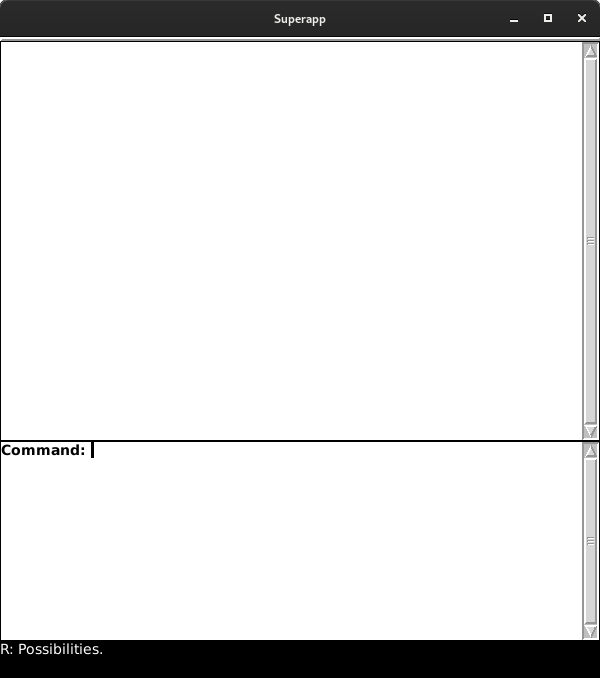
\includegraphics[width=.6\linewidth]{ex2-screenshot.png}
\end{center}
\caption{\label{ex2} View of the improved example}
\end{figure}

Notice that commands, in order to be available from the command line,
must have an option of \texttt{:name t}.  The reason is that some
commands will be available only from menus or by some other mechanism.

You may notice that if the output of the application is hidden (say by
the window of some other application) and then re-exposed, the output
reappears normally, without any intervention necessary on the part of
the programmer.  This effect is accomplished by a CLIM mechanism
called \emph{output recording}.  Essentially, every piece of output is
not only displayed in the pane, but also captured in an \emph{output
  record} associated with the pane.  When a pane is re-exposed, its
output records are consulted and if any of them overlap the re-exposed
region, they are redisplayed.  In fact, some others may be redisplayed
as well, because CLIM guarantees that the effect will be the same as
when the initial output was created.  It does that by making sure that
the order between (partially) overlapping output records is respected.

Not all panes support output recording, but certainly application
panes do, so it is good to use some subclass of
\texttt{application-pane} to display application-specific object,
because output recording is then automatic.

\section{An application displaying a data structure}

Many applications use a central data structure that is to be on
display at all times, and that is modified by the commands of the
application.  CLIM allows for a very easy way to write such an
application.  The main idea is to store the data structure in slots of
the application frame, and to use a \emph{display function} that after
each iteration of the command loop displays the entire data structure
to the application pane.

Here is a variation of the previous application that shows this
possibility, and in which the \texttt{parity} command is now useful.

\verbatiminput{ex2b.lisp}

Here, we have added a slot that is called \texttt{current-number} to
the application frame.  It is initialized to \texttt{NIL} and it has
an accessor function that allows us to query and to modify the value.

Observe that in this example, we no longer have the option
\texttt{:display-time nil} set in the application pane.  By default,
then, the \texttt{:display-time} is \texttt{:command-loop} which means
that the pane is erased after each iteration of the command loop.
Also observe the option \texttt{:display-function} in the application
pane definition which takes a symbol that names a function to be
called to display the pane after it has been cleared.  In this case,
the name is \texttt{display-app}, the name of the function defined
immediately after the application frame.

Instead of immediately displaying information about its argument, the
command \texttt{com-parity} instead modifies the new slot of the
application frame.  Think of this function as being more general, for
instance a command to add a new object to a set of graphical objects
in a figure drawing program, or as a command to add a new name to an
address book.  Notice how this function accesses the current
application frame by means of the special variable
\texttt{*application-frame*}.

A display function is called with the frame and the pane as arguments.
It is good style to use the pane as the stream in calls to functions
that will result in output.  (Recall that a pane is a stream of
rendering instructions.) This makes it possible for the same function
to be used by several different frames, should that be called for.  In
our simple example, the display function only displays the value of a
single number (or \texttt{NIL}), but you could think of this as
displaying all the objects that have been drawn in some figure drawing
program or displaying all the entries in an address book.

\section{Incremental redisplay}

While the example in the previous section is a very simple way of
structuring an application (let commands arbitrarily modify the data
structure, and simply erase the pane and redisplay the structure after
each iteration of the command loop), the visual result is not so great
when many objects are to be displayed.  There is most often a
noticeable flicker between the moment when the pane is cleared and the
objects are drawn.  Sometimes this is inevitable (as when nearly all
objects change), but most of the time, only an incremental
modification has been made, and most of the objects are still in the
same place as before. E.g. no point refreshing a whole spreadsheet
when only a single cell's content has changed.

In simpler GUI toolkits, the application programmer would have to
provide code logic to explicitly track what might changed since the
previous display, and only display the differences.  CLIM offers a
mechanism called \emph{incremental redisplay} that automates a large
part (but not all) of this task.  As we mentioned earlier, CLIM can
transparently and continuously capture output in the form of
\emph{output records}.  The same mechanism is used to obtain
incremental redisplay.

The incremental redisplay code of a pane remains structured as in the
previous section: after each iteration of the command loop, the
display function needs to produce an output (the rendering
instructions) of the entire data structure. As before, the new
(incremental) display code will iterate through each individual
element of that pane, but this time with a way to test whether this
element has changed. The mechanics of updating the internal structure
of the output, changing only needs to be changed, is then fully
handled by CLIM: instead of regenerating the entire stream of
instructions to render a particular pane, only the instructions of a
modified element of that pane will be updated and only part of that
stream of instructions will be modified.

To achieve this, each element of that pane is given a unique
identifier, as well as a way to compare the value referenced by that
identifier before and after a redisplay request.  The incremental
redisplay mechanism then works by telling CLIM which piece of output
corresponds to which piece of output during the previous iteration of
the command loop. With this information, the CLIM incremental
redisplay mechanism can figure out whether some output is new, has
disappeared, or has been moved, compared to the previous iteration of
the command loop.  As with re-exposure, CLIM guarantees that the
result is identical to that which would have been obtained, had all
the output records been output in order to a blank pane.

The next example illustrates this idea.  It is a simple application
that displays line-by-line a list of random numbers (here 20). The
user is then able to move a cursor represented by a star at the
beginning of a line, and increase or decrease the number on that line
by 1.

When displaying those lines (displaying the first time or refreshing
the display afterwards), the code will identify which has changed or
not, and only update the \texttt{output record} (the list of rendering
instructions) if a number changed. Concretely, moving the star cursor
up or down does not modify the number and therefore should not affect
the \texttt{output record} of that number; this should only happen
when a number is increased or decreased. The star cursor however will
always be re-rendered without using the incrementaly redisplay
mechanics.


Here is the code achieving this:

\verbatiminput{ex2c.lisp}

We store the numbers in a slot called \texttt{numbers} of the
application frame.  However, we store each number in its own list.
This is a simple way to provide a unique identity for each number.  We
could not use the number itself, because two numbers could be the
same. Since numbers evaluate to themselves, the identities would not
be unique.  Instead, we use the cons cell that store the number as the
unique identity.  By using \texttt{:id-test \'eq} we inform CLIM that
it can figure out whether an output record is the same as one that was
issued previous time by using the function \texttt{eq} to compare
them.  But there is a second test that has to be verified, namely
whether an output record that was issued last time has to be
redisplayed or not.  That is the purpose of the cache-value.  Here we
use the number itself as the cache value and \texttt{eql} as the test
to determine whether the output is going to be the same as last time.

For convenience, we display a \texttt{*} at the beginning of the
current line, and we provide two commands \texttt{next} and
\texttt{previous} to navigate between the lines. The command
\texttt{add} increases the value of the number at the cursor position.

Notice that in the declaration of the pane in the application frame,
we have given the option \texttt{:incremental-redisplay t}.  This
informs CLIM not to clear the pane after each command-loop iteration,
but to keep the output records around and compare them to the new ones
that are produced during the new iteration.
